\documentclass{beamer}
\mode<presentation>
{
  \usetheme{default}      % or try Darmstadt, Madrid, Warsaw, ...
  \usecolortheme{default} % or try albatross, beaver, crane, ...
  \usefonttheme{default}  % or try serif, structurebold, ...
  \setbeamertemplate{navigation symbols}{}
  \setbeamertemplate{caption}[numbered]
} 

\usepackage{graphics}
\usepackage[english]{babel}
\usepackage[utf8]{inputenc}
%\usepackage[T1]{fontenc}
\usepackage{biblatex}
\usepackage{adjustbox}
\usepackage{caption}
%\usepackage{algorithm2e}
\usepackage{algorithm}
\usepackage{algorithmic}
\usepackage{tikz-cd}
\usepackage{graphicx}
\usepackage{subfig}
\usetikzlibrary{arrows.meta,
                positioning
                }
                
%\usepackage{beamerthemesplit}

\captionsetup[figure]{labelformat=empty}% redefines the caption setup of the figures environment in the beamer class.

%\usepackage{natbib}
%\bibliographystyle{apalike} 
\bibliography{bibsamp.bib}
%\usepackage{bibentry}
%\usepackage{natbib}

%\usepackage{filecontents}
%\addbibresource{bibsamp.bib}

%\nobibliography*
%\usepackage{comment}
%\usepackage{booktabs}
%\usepackage{afterpage}
%\usepackage{makecell}
%\usepackage{fourier} 
%\usepackage{array}
%\usepackage{xr}
%\usepackage{cleveref}

%\setbeamertemplate{caption}{\raggedright\insertcaption\par}

\title[Modelling the cell-type specific murine connectome]{Modelling the cell-type specific mesoscale murine connectome}
\author{Samson Koelle}
\institute{Allen / UW Department of Statistics}
\date{1/20/21}

\begin{document}

\begin{frame}
  \titlepage
\end{frame}

%Uncomment these lines for an automatically generated %outline.
%\begin{frame}{Outline}
% \tableofcontents
%\end{frame}

\section{Introduction}

\begin{frame}{Us : first meeting - Neurips ( Dec 2019)}
\begin{columns}
\begin{column}{0.33\textwidth}
Allen Brain
\begin{figure}
    \centering
    \includegraphics[width = 1.2in]{figs/figsforpres/stefan.jpg}
    \caption{Stefan Mihalas}
\end{figure}
\begin{itemize}
    \item Julie Harris
    \item Jennifer Whitesell
\end{itemize}

\end{column}
\begin{column}{.33\textwidth}
UW Statistics
\begin{figure}
    \centering
    \includegraphics[width = 1in]{figs/figsforpres/meila.jpeg}
    \caption{Marina Meila - Professor of Statistics}
\end{figure}

\begin{figure}
    \centering
    \includegraphics[width = 1in] {figs/figsforpres/koelle_linkedin.png}
    \caption{K - 6th year PhD  (unsupervised learning)}
\end{figure}
\end{column}
\end{columns}
\end{frame}

\begin{frame}{Recent work}
\begin{itemize}
    \item \fullcite{Oh2014-kh}
    \item \fullcite{Harris2016-fn}
    \item \fullcite{Knox2019-ot}
    \item \fullcite{Harris2019-mr}
\end{itemize}
\end{frame}

\begin{frame}{Anterograde tracing experiments}
\begin{figure}
    \centering
    \includegraphics[width = 4in]{figs/figsforpres/oh2014figure1.jpg}
    \caption{\citeauthor{Oh2014-kh}}
    \label{fig:my_label}
\end{figure}
\end{frame}

\begin{frame}{Modelling connectivities}
\begin{itemize}
    \item Modelling = combining data from different experiments.
\item A connectivity model estimates 
\begin{eqnarray*}
\mathcal C: S \times T \to \mathbb R_{\geq 0},
\end{eqnarray*}
the matrix containing connection from \textit{source} $s \in S$ to \textit{target} $t \in T$.  
\end{itemize}

\begin{table}
    \centering
    \begin{adjustbox}{width=.8\columnwidth,center}
    \begin{tabular}{c|c|c|c}
        Paper & Model & $\mathcal S$ , $\mathcal T $ & Cre \\
         \hline
        \citet{Oh2014-kh} & Structure non-negative linear regression & Structures & N \\
        \citet{Harris2016-fn}  & Splines & Voxels & N   \\
        \citet{Knox2019-ot} & Voxel Nadaraya-Watson &   Structures  &   N
        \end{tabular}
    \end{adjustbox}
    \caption{Modelling approaches}
    \label{tab:my_label}
\end{table}
\end{frame}

\begin{frame}{Cre-specific targeting}
\begin{itemize}
    \item Key idea: mice express Cre recombinase in certain cell-lines
    \item AAV requires Cre for expression of GFP
\end{itemize}
\begin{figure}
    \centering
    \includegraphics[width = 2.5in]{figs/figsforpres/Screen Shot 2021-01-18 at 10.05.27 PM.png}
    \caption{\citeauthor{Harris2019-mr}}
    \label{fig:my_label}
\end{figure}
\end{frame}


\begin{frame}{Our goal}
The goal is to use tracing experiments from \citeauthor{Harris2019-mr} to estimate 
\begin{eqnarray*}
\mathcal C: V \times S \times T \to \mathbb R_{\geq 0},
\end{eqnarray*}
the matrix containing connection from \textit{source} $s \in S$ to \textit{target} $t \in T$ observed with virus  $v$.
\end{frame}

\section{Data}

\begin{frame}{An example experiment}
\begin{figure}
    \centering
    \includegraphics[width = 4in]{figs/figsforpres/inj_proj_figure.png}
    \caption{Example of experimental data}
    \label{fig:my_label}
\end{figure}
\end{frame}

\begin{frame}{Experimental data}
For each experiment $i$, we have access (AllenSDK) to 
\begin{itemize}
    \item Cre-line $v(i) \in V$
    \item Injection $x(i) \in \mathcal B \subset \mathbb R^{130 \times 75 \times 102}$
    \item Projection $y(i) \in \mathcal B $
    \item Data quality mask $q(i) \in \mathcal B$ (use threshold)
    \item Injection fraction mask $l(i) \in \mathcal B$
\end{itemize}
We can then compute
\begin{itemize}
    \item Weighted injection centroid $c(i) \in \mathbb R^3$
    \item Regionalization maps $r(i) \in \mathbb R^{|S|}$ or $\mathbb R^{|T|}$
\end{itemize}
\end{frame}

\begin{frame}{Regionalizations}
%Size of $T$, $S$
\begin{itemize}
    \item Many choices of regionalization map
    \item Convention: $S$ ipsilateral
\end{itemize}
\begin{figure}
    \centering
    \includegraphics[width = 3.5in]{figs/figsforpres/ontologyfigure.png}
    \caption{Regionalization options in Allen SDK}
    \label{fig:my_label}
\end{figure}
\end{frame}

\begin{frame}{Dataset}
\begin{columns}
\begin{column}{.5\textwidth}
\begin{figure}
    \centering
    \includegraphics[width = 2in]{figs/figsforpres/datasummary.png}
    \caption{Data summary}
    \label{fig:my_label}
\end{figure}
\end{column}
\begin{column}{.5\textwidth}
\begin{figure}
    \centering
    \includegraphics[width = 2in]{figs/figsforpres/visp_counts.png}
    \caption{Heterogenous distribution of injection centroids}
    \label{fig:my_label}
\end{figure}
\end{column}
\end{columns}
\end{frame}

\begin{frame}[fragile]{Data preprocessing}
%\begin{itemize}
%    \item $T = \text{Summary structures}$
%\end{itemize}
% cre abundances, structure abundances, loss

%\begin{adjustbox}{width=.8\columnwidth,center}
%\begin{algorithmic}
\begin{minipage}{1.\linewidth}

\begin{algorithm}[H]{Injection $x(i)$, projection $y(i)$,  injection fraction $l(i)$, quality mask $q(i)$, regionalization map $r: \mathcal B \to T$}
\algsetup{linenosize=\tiny}
\scriptsize
\begin{algorithmic}[1]
%\State Here
%\begin{algorithm}[H]
\STATE Adjust for injection fraction $x_l (i) = l(i) \odot y(i)$
\STATE Data-quality censor $y_q (i) = y (i) \odot q(i), x_q(i) = x_l (i) \odot q(i)$
\STATE Compute weighted injection centroid $c(i) := c(x_q(i))$
\IF {$c(i) \in \mathcal B_{left}$}
 \STATE Flip $c(i), y_q (i), x_q(i)$
\ENDIF 
%(also $x_M(i) = M(i) \odot x(i)$ for linear model)
%\STATE Normalize $x_N(i) = F(i) \odot x_M(i)$ (only for linear model)
\STATE Average/sum structures $y_r (i) = r(y_q (i))$% (also $x_S (i) = A x_M(i)$ for linear model)
\STATE Normalize $ y_n(i) = \frac{y_r (i)}{\|y_r (i)\|}$ (new) %(also $\tilde x (i) = A x_M(i)$ for linear model)
\RETURN $ y_n(i), c(i)$ (optional $x_r = r( x_q(i))$ )
\end{algorithmic}
\end{algorithm}
%\end{adjustbox}
\end{minipage}
%\end{algorithmic}
%\end{adjustbox}
\end{frame}

\begin{frame}{The centroid Nadaraya-Watson model (\citeauthor{Knox2019-ot})}
\begin{itemize}
    \item $\hat f_M^{NW} := \text{NW}  (c(I_M),  y_r(I_M))$ outperforms $\hat f_M^{NNLR} :=  \text{NNLR}(x_r(I_M), y_r(I_M)$) 
    \item $I_M := $ experiments in a major brain division
\end{itemize}
\begin{figure}
    \centering
    \includegraphics[width = 4in]{figs/figsforpres/Screen Shot 2021-01-19 at 5.53.58 PM.png}
    \caption{\citeauthor{Knox2019-ot}}
    \label{fig:my_label}
\end{figure}
\begin{itemize}
    \item $\hat  f_M^{NW}$ is inherently an improvement on the naive model $\hat \mu_M$ that averages over $I_M$ due to selection of bandwidth $\gamma$.
\end{itemize}
\end{frame}


\begin{frame}{Cre-specific NW}
\begin{itemize}
    \item A simple cre-specific candidate model is $\hat f_{s, v}^{NW} = NW (c(I_{s, v}),  y_r(I_{s, v}))$)
    \item $I_{s, v}$ are the experiments sharing a structure and virus.
    \item Should reap substantial benefits going from $240$ to $1751$ experiments.
    \item Problem: small $|I_{s, v}|$ can hamper estimation
    \item Key idea: include experiments with similar $v$ in model.
    %is therefore $NW$ on cre-structure combinations (e.g. $\hat f_{M, v} = NW (c(I_{M, v}),  y_r(I_{M, v}))$)
   % \item We may wish to restrict to summary structure or leaf-specific smoothing (e.g. 
\end{itemize}
\end{frame}

\begin{frame}{Expected-loss model}

\begin{columns}
\begin{column}{0.5\textwidth}
\begin{adjustbox}{width=1.2\columnwidth,center}
%\begin{figure}
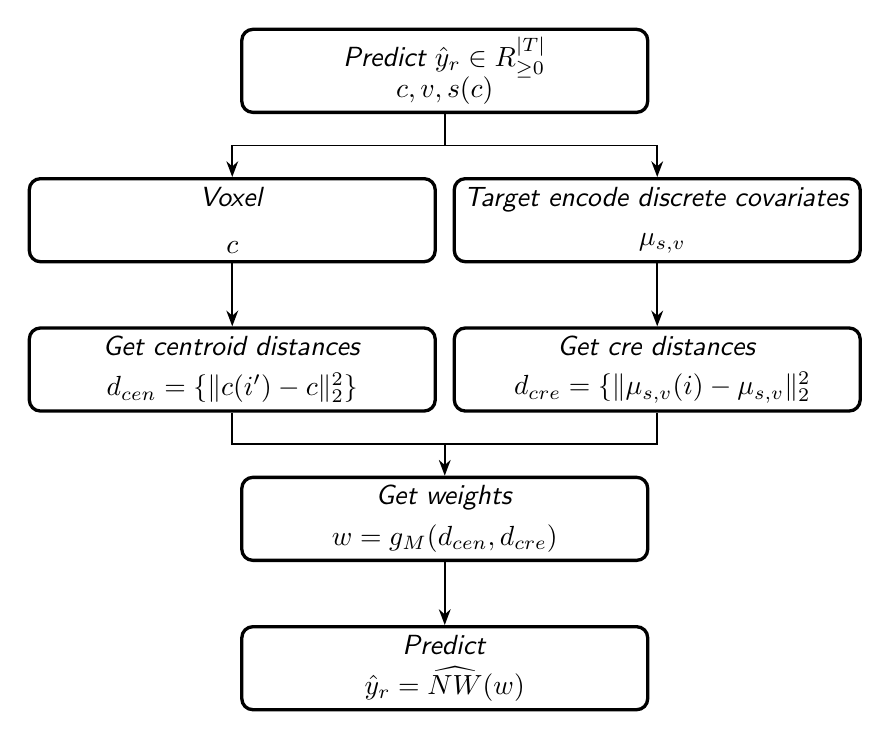
\begin{tikzpicture}[
  node distance = 8mm and 1mm,
job/.style args = {#1/#2}{
    rectangle, rounded corners, draw=black, very thick,
    minimum height=3em, text width=14em, align=center,
    label={[font=\sffamily,anchor=north]above:\textit{#1}},
    label={[font=\sffamily,anchor=south]below:\textbf{#2}},
    node contents ={}},
    arr/.style = {semithick, -Stealth}
                    ]
\node (n1)  [job=Predict ${\hat y_r \in \mathbb R_{\geq 0}^{|T|}}$/${c, v, s(c)}$];
\node (n21) [job=Voxel /$c$,below left=of n1.south];%$c(i)$/ 2 ,below  left=of n1.south];
\node (n22) [job= Target encode discrete covariates/ ${\mu_{s,v}} $,below right=of n1.south];%$v(i), s(i)$/compute mean $\mu_{s,v}$,below right=of n1.south];
\node (n31) [job=Get centroid distances/${d_{cen} = \{\|c(i') - c\|_2^2 \}} $,below =of n21.south];%$c(i)$/ 2 ,below  left=of n1.south];
\node (n32) [job= Get cre distances/ ${d_{cre} =\{\|\mu_{s,v}(i) - \mu_{s,v}\|_2^2  } $,below =of n22.south];%$v(i), s(i)$/compute mean $\mu_{s,v}$,below right=of n1.south];

\node (n4)  [job=Get weights/${w  = g_M({d_{cen}, d_{cre}})}$,below right=of n31.south];
\node (n5)  [job= Predict/{$\hat y_r = \widehat{NW}(w)$},below=of n4];
%
\coordinate[below=4mm of n1.south] (aux1);
\coordinate[above=4mm of n4.north] (aux2);
%
\draw[arr]  (n1) -- (aux1) -| (n21);
\draw[arr]  (aux1) -| (n22);
\draw[arr]  (n22) -- (n32);
\draw[arr]  (n21) -- (n31);
\draw[arr]  (n31) |- (aux2)
            (n32) |- (aux2) -- (n4);
\draw[arr]  (n4)  -- (n5);
%\caption{2+2}
   \end{tikzpicture}
  
   %\caption{2+2}
%\end{figure}
  \end{adjustbox}
\end{column}
\begin{column}{0.5\textwidth}
\begin{figure}
    \centering
    \includegraphics[width = 1in]{figs/figsforpres/315_summary_scatter.png}
    \caption{Isocortex loss distribution}
    \label{fig:my_label}
\end{figure}
\begin{figure}
    \centering
    \includegraphics[width = 1in]{figs/figsforpres/315_summary_surface.png}
    \caption{$\hat g$ fit to expected-loss using shape-constrained splines}
    \label{fig:my_label}
\end{figure}
\end{column}
\end{columns}
\end{frame}

\begin{frame}{Model evaluation}
\begin{itemize}
    \item Naive leave-one-out cross-validation (\citeauthor {Knox2019-ot})
    \begin{eqnarray*}
    \mathcal{L} ( \hat f) = \frac{1}{|I_M|} \sum_{i \in I_M} \| y_r(i) - \hat f(c(i)) \|_2^2 
    \end{eqnarray*}
    \item Weighted leave-one-out cross-validation
    \begin{eqnarray*}
    \mathcal{L} ( \hat f) = \frac{1}{|\{S,V\}|} \sum_{s,v \in \{S,V\}} \frac{1}{ |I_{s,v}|} \sum_{i \in I_{s,v} } \| y_r(i) - \hat f(c(i)) \|_2^2 
    \end{eqnarray*}
    \item Evaluation set determined by most restrictive smoothing (requires $|I| > 1$).%$\{\{I_M\}$ or $\{I_{s,v}\}$ determined by most restrictive model $|I| > 1$
\end{itemize}
\end{frame}

%\section{Results}
\begin{frame}{Model selection}
\begin{itemize}
    \item EL model performs best over a range of objectives (unweighted/weighted loss, leaf/summary (SS) targets) 
    \item and smoothings (major (M)/SS/leaf))
\end{itemize}
%results for summary average
%results for NW
%results for EL
\begin{table}
\begin{adjustbox}{width=.7\columnwidth,center}

\begin{tabular}{ll|rrrrr}
\toprule
   & Estimator &     EL &     NW & Average &     NW &  NW-wt \\
   & Smoothing &     SS & Cre-SS &  Cre-SS &     SS &      M \\
   & Target &     SS &     SS &      SS &     SS &     SS \\
Structure & \# Eval exps &        &        &         &        &        \\
\midrule
\hline
CB & 10 &  0.044 &  0.081 &   0.081 &  0.058 &  0.439 \\
CTXsp & 2 &  0.497 &  0.497 &   0.497 &  0.497 &  0.000 \\
HPF & 79 &  0.122 &  0.140 &   0.143 &  0.155 &  0.471 \\
HY & 41 &  0.241 &  0.266 &   0.269 &  0.244 &  1.019 \\
Isocortex & 838 &  0.173 &  0.195 &   0.202 &  0.234 &  0.404 \\
MB & 23 &  0.151 &  0.151 &   0.166 &  0.139 &  0.759 \\
MY & 7 &  0.186 &  0.233 &   0.233 &  0.184 &  0.452 \\
OLF & 17 &  0.069 &  0.095 &   0.100 &  0.073 &  0.110 \\
P & 8 &  0.236 &  0.239 &   0.239 &  0.264 &  0.984 \\
PAL & 11 &  0.190 &  0.198 &   0.198 &  0.260 &  1.401 \\
STR & 45 &  0.084 &  0.088 &   0.089 &  0.097 &  0.265 \\
TH & 29 &  0.351 &  0.678 &   0.678 &  0.365 &  1.088 \\
\bottomrule
\end{tabular}
\end{adjustbox}
\caption{e.g. weighted losses }
\end{table}

\end{frame}

\begin{frame}{Model performance details}
\begin{itemize}
    \item Provide detailed model-performance information to calibrate user confidence
\end{itemize}
\begin{figure}
    \centering
    \includegraphics[width = 3in]{figs/figsforpres/loss_details.png}
    \caption{Structure/cre-specific losses for EL in isocortex.}
    \label{fig:my_label}
\end{figure}
\end{frame}

\begin{frame}{Constructing connectivities}

\begin{itemize}
    \item Connectivities are constructed as in \citeauthor{Knox2019-ot} by summing or averaging over each structure $s$:
\end{itemize}
\begin{eqnarray*}
\mathcal C_{v,s} = \sum_{c \in s} \widehat{EL} (c,v,s)
\end{eqnarray*}
\end{frame}

\begin{frame}{Estimated wild-type connectivity}
%\begin{center}
%\hspace{-10in}
\begin{figure}[H]
    \centering
    \includegraphics[width = 4.5in]{figs/figsforpres/Figure2.png}
    \caption{Now with lower loss!}
    \label{fig:my_label}
\end{figure}
%\end{center}
\end{frame}

\begin{frame}{Cell-type examples}

\begin{figure}
    \centering
    \includegraphics[width = 4in]{figs/visp_mo_1201.png}
    \caption{Reproduces results of \citet{Jeong2016-dc} (non-Allen)}
    \label{fig:my_label}
\end{figure}
\end{frame}

\begin{frame}{Clustering connectivity by cell-type}
\begin{figure}
    \centering
    \includegraphics[width = 3in]{figs/Figure4.png}
    \caption{Behavior clusters by cell-type in expected way}
    \label{fig:my_label}
\end{figure}
\end{frame}

\begin{frame}{Factoring the wild-type connectome with NMF}
\begin{itemize}
    \item Non-negative matrix factorization:
\end{itemize}
\begin{eqnarray*}
\arg \min_{W,H} \|\hat{  \mathcal C}  - WH  \|_{\text{dist}\geq 1500 \mu m}^2
\end{eqnarray*}
    \begin{figure}
    \centering
\subfloat[Distances between regions \label{fig:1}]{
    \includegraphics[width=0.35\textwidth]{figs/figsforpres/distances.png}}
\subfloat[CV for NMF for distal connectivites \label{fig:2}]{
    \includegraphics[width=0.3\textwidth]{figs/figsforpres/test_train.png}}
\subfloat[Top connectivity components \label{fig:2}]{
    \includegraphics[width=0.35\textwidth]{figs/figsforpres/components.png}}
\caption{Caption.}
\label{fig:caption}
    \end{figure}
\end{frame}

\begin{frame}{Publication plan}
\begin{itemize}
    \item Connectivities used in "Distinct organization of functional connectivity along different frequency bands across visual cortical area" - submitted (w/ Zachary Taylor, Stefan)
    \item Manuscript under preparation for Network Neuroscience.
    \item Investigating other collaborations.
\end{itemize}
\end{frame}

\begin{frame}{Conclusion and future work}
\begin{itemize}
    \item We can generate smoothed, cell-type connectivity matrices in the manner of \citeauthor{Knox2019-ot} for the \citeauthor{Harris2019-mr} data set that correspond to the expected biology.
    \item We have developed a well-performing new model
    %\item The resultant connectivities .
    \item Main product: connectivities, model evaluation information, easy to use / flexible software
    \item Secondary product: proof-of-concept unsupervised analyses
    \item Future questions: Is there a better loss for our data $\in \mathbb R_{\geq 0}$? How else should the connectivity tensor be analyzed? How can we combine $NNLR$ and $NW$ or $EL$?
    \item Other things we've tried: estimating sparsity, factorizing $x$ and $y$ in model.
\end{itemize}
\end{frame}

\begin{frame}{Thank you!}
Questions?
\end{frame}






\end{document}
